\documentclass{article}

% Formatting
\usepackage[utf8]{inputenc}
\usepackage[margin=1in]{geometry}
\usepackage[titletoc,title]{appendix}
\usepackage[spanish]{babel}
\usepackage{amsmath,amsfonts,amssymb,mathtools}
\usepackage{graphicx,float}
\usepackage[ruled,vlined]{algorithm2e}
\usepackage{algorithmic}
\usepackage{minted}
\usemintedstyle{borland}
\usepackage{biblatex}

% Title content
\title{Práctica 1 Movimiento Brawniano}
\author{Denisse leyva}
\date{Febrero 17, 2021}

\begin{document}

\maketitle

% Introduction
\section{Introducción}
En esta practica número 1 se trata el tema Movimiento Brawniano de una partícula, se debe analizar el tiempo de regreso al origen de dicha particula en diferentes dimensiones (de 1 a 5) en incrementos lineales, variando el numero de pasos de la caminata como potencias de dos con exponente de 4 a 9 en  incrementos lineales de uno, con 30 repeticiones del experimento para cada combianción.  


\section{Objetivo}
El objetivo de la simulación es verificar por medio de las 5 dimensiones y las 30 repeticiones en cada cantidad de pasos especifica cuanto se tarda la particula en regresar al origen o si no regresa nunca. 
Y graficar los datos resultantes en un diagrama caja-bigote asi como obtener un cuadro con la información del minimo, promedio y maximo del tiempo de regreso para cada dimensión asi como el porcentaje de las que nunca regresaron.


\section{Código}
En el siguiente código se utilizaron secuencias for para realizar todo el objetivo propuesto en una sola ejecución.
Todo esta centrado en el primer for que determina la cantidad de pasos. En el segundo for se determina la dimensión a trabjar con el número de pasos que arrojo el for anterior. En el tercer for se especifican las repeticiones para cada dimensión.\\
Ademas se utilizó la libreria pandas para crear las tablas con el mínimo, promedio, máximo y el porcentaje de las partículas que nunca regresaron al origen.\\


Código creado en Python\\
\begin{verbatim}
from random import random, randint
import matplotlib.pyplot as plt 
import pandas as pd


for e in range(6):
    exponencial = e + 4
    exp = 2 ** exponencial
    print('Con numero de pasos de ', exp)
    rf=[],[],[],[],[]
    minimo, maximo, promedio, porcentaje = [],[],[],[]
    for d in range(5):
        dimension = d+1
        p_inicial = [0] * dimension
        resultados = []
        resultados1 = []
        repeticiones = 30
    
        for nr in range(repeticiones):
            nunca = True
    
            for paso in range(exp):
                dim = randint(0, dimension-1)
                p_inicial[dim] = p_inicial[dim] + 1 if random() < 0.5 else p_inicial[dim] -1
                
                if all([p == 0 for p in p_inicial]):
                    resultados.append(paso+1)
                    resultados1.append(paso+1)
                    nunca = False
                    break
            if nunca:
                resultados.append(None)
                # resultados1.append(exp+1)
        
        cuantos = sum([r is None for r in resultados])
        # print((cuantos / repeticiones)*100, 'no regresaron nunca en la dimension ', d+1)
        porcentaje.append((cuantos / repeticiones)*100)
        if cuantos < repeticiones:
            regresaron = sum([r if r is not None else 0 for r in resultados])
            # print(regresaron / (repeticiones - cuantos), 'fue la tardanza en promedio en la dimension ', d+1)
        for r in resultados1:
            rf[d].append(r) 
        # print(rf[d])
        if rf[d] > []:
            mi = min(rf[d])
            prom = sum(rf[d])/len(rf[d])
            ma = max(rf[d])
            minimo.append(mi)
            promedio.append(prom)
            maximo.append(ma)
        else:
            # print("se anula")
            minimo.append('Anulado')
            promedio.append('Anulado')
            maximo.append('Anulado')
        
            
    data = {'Dimension':[1,2,3,4,5], 
            'Minimo':minimo, 
            'Promedio':promedio, 
            'Maximo':maximo,
            'Porcentaje':porcentaje} 
    # print(data)
    df = pd.DataFrame(data)
    print(df)
        
    fig, ax = plt.subplots()
    ax.boxplot(rf)
    ax.set_xlabel('Dimensión')
    ax.set_ylabel('Pasos')
    ax.set_title('Total de Pasos: ' + str(exp))
    # ax.set_title('')
    plt.savefig('p1_pasos_de_'+ str(exp) + '.png')
    # plt.close()
\end{verbatim}

% Computational Results
\section{Resultados}
En las Figuras de la 1 a la 6 se muestra un diagrama caja-bigote con los datos de las partículas que regresaron al origen con los pasos determiandos en la caminata.

\begin{figure}[H]
\centering
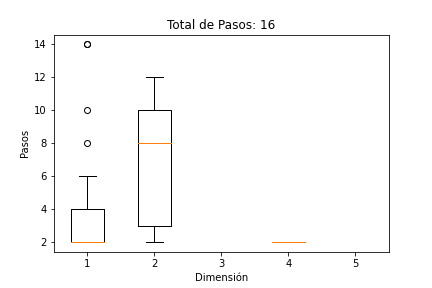
\includegraphics[width=80mm]{p1_pasos_de_16.png}
\caption{\label{fig1}Caminata 16 pasos.}
\end{figure}
\begin{figure}[H]
\centering
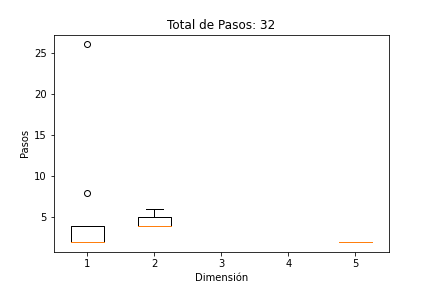
\includegraphics[width=80mm]{p1_pasos_de_32.png}
\caption{\label{fig1}Caminata 32 pasos.}
\end{figure}
\begin{figure}[H]
\centering
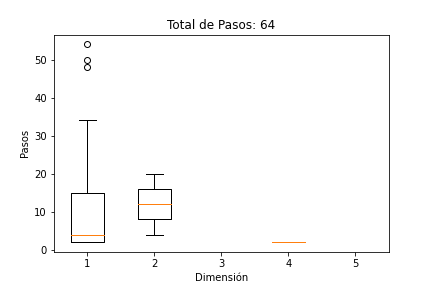
\includegraphics[width=80mm]{p1_pasos_de_64.png}
\caption{\label{fig1}Caminata 64 pasos.}
\end{figure}
\begin{figure}[H]
\centering
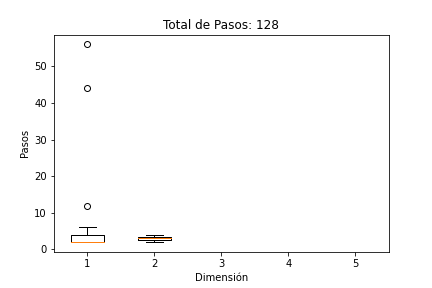
\includegraphics[width=80mm]{p1_pasos_de_128.png}
\caption{\label{fig1}Caminata 128 pasos.}
\end{figure}
\begin{figure}[H]
\centering
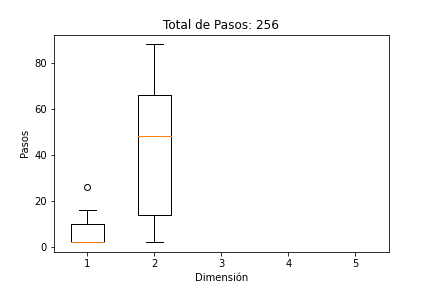
\includegraphics[width=80mm]{p1_pasos_de_256.png}
\caption{\label{fig1}Caminata 256 pasos.}
\end{figure}
\begin{figure}[H]
\centering
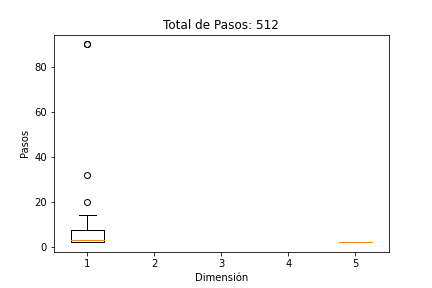
\includegraphics[width=80mm]{p1_pasos_de_512.png}
\caption{\label{fig1}Caminata 512 pasos.}
\end{figure}

En las figuras de la 7 a la 12 se muestran las tablas con el mínimo el promedio el máximo y el porcentaje de las partículas que regresaron al origen.

\begin{figure}[H]
\centering
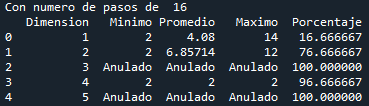
\includegraphics[width=80mm]{tabla_pasos16.png}
\caption{\label{fig1}Caminata 16 pasos.}
\end{figure}
\begin{figure}[H]
\centering
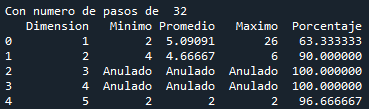
\includegraphics[width=80mm]{tabla_pasos32.png}
\caption{\label{fig1}Caminata 32 pasos.}
\end{figure}
\begin{figure}[H]
\centering
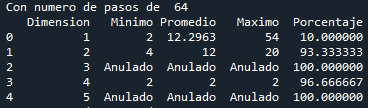
\includegraphics[width=80mm]{tabla_pasos64.png}
\caption{\label{fig1}Caminata 64 pasos.}
\end{figure}
\begin{figure}[H]
\centering
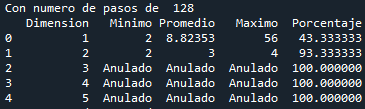
\includegraphics[width=80mm]{tabla_pasos128.png}
\caption{\label{fig1}Caminata 128 pasos.}
\end{figure}
\begin{figure}[H]
\centering
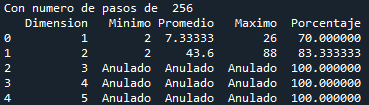
\includegraphics[width=80mm]{tabla_pasos256.png}
\caption{\label{fig1}Caminata 256 pasos.}
\end{figure}
\begin{figure}[H]
\centering
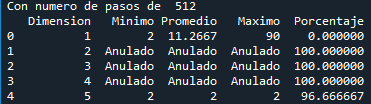
\includegraphics[width=80mm]{tabla_pasos512.png}
\caption{\label{fig1}Caminata 512 pasos.}
\end{figure}


 
\section{Reto 1}
El primer reto es estudiar de forma sistemática y automatizada el tiempo de ejecución de una caminata (en milisegundos), en términos de largo de la caminata (en pasos) y la dimensión. Para medir el tiempo de una replica, se debe ejecutar multiples vecesy normalizar con la cantidad de repeticiones para obtener un promedio del tiempo de una replica individual.[1]

Para este reto se modificó el número de repetciones aumentadolo a 500 para tener mas numeros de muestras y obtener un buen promedio,tambien se agrego una variable que guarda el tiempo inicial y una que guarda el tiempo final en milisegundos, con estas dos variables se determinó el tiempo que trabaja la caminata y solo se promedio con el número de repeticiones.
Ademas se agrego un conteo de pasos totales ya que este si cuenta con los pasos completos aunque no acabe el recorrido de regreso a cero para obtener un promedio de los pasos totales por caminata.

\begin{verbatim}

from random import random, randint
import matplotlib.pyplot as plt 
import pandas as pd
import time


for e in range(6):
    exponencial = e + 4
    exp = 2 ** exponencial
    print('Con numero de pasos de ', exp)
    rf=[],[],[],[],[]
    minimo, maximo, promedio, porcentaje, tiempo_t, pasos_c= [], [], [], [], [], []
    for d in range(5):
        dimension = d+1
        p_inicial = [0] * dimension
        resultados = []
        resultados1 = []
        repeticiones = 500
        inicio = time.time()
        p_t = []
        
        for nr in range(repeticiones):
            nunca = True
                        
            for paso in range(exp):
                dim = randint(0, dimension-1)
                p_inicial[dim] = p_inicial[dim] + 1 if random() < 0.5 else p_inicial[dim] -1
                
                if all([p == 0 for p in p_inicial]):
                    resultados.append(paso+1)
                    resultados1.append(paso+1)
                    nunca = False
                    break
            p_t.append(paso+1)
            if nunca:
                resultados.append(None)
                # resultados1.append(exp+1)
        
         
        final = time.time()
        tiempo = final - inicio
        tiempo_p = tiempo/repeticiones
        tiempo_t.append(tiempo_p)
        # print("tiempo promedio de caminata: ",tiempo_p, " en la dimension: ", dimension)
        prom_pasos = sum(p_t)/repeticiones
        pasos_c.append(prom_pasos)
        # print("el promedio de pasos completos es: ",pasos_c)
        
        cuantos = sum([r is None for r in resultados])
        # print(cuantos , "no regresaron")
        # print((cuantos / repeticiones)*100, 'no regresaron nunca en la dimension ', d+1)
        porcentaje.append((cuantos / repeticiones)*100)
        if cuantos < repeticiones:
            regresaron = sum([r if r is not None else 0 for r in resultados])
            # print(regresaron)
            # print(regresaron / (repeticiones - cuantos), 'fue la tardanza en promedio en la dimension ', d+1)
        for r in resultados1:
            rf[d].append(r) 
        # print(rf[d])
        if rf[d] > []:
            mi = min(rf[d])
            prom = sum(rf[d])/len(rf[d])
            ma = max(rf[d])
            minimo.append(mi)
            promedio.append(prom)
            maximo.append(ma)
        else:
            # print("se anula")
            minimo.append('Anulado')
            promedio.append('Anulado')
            maximo.append('Anulado')
        
            
    data = {'Dimension':[1,2,3,4,5], 
            'Minimo':minimo, 
            'Promedio':promedio, 
            'Maximo':maximo,
            'Porcentaje':porcentaje,
            'Tiempo_promedio' : tiempo_t} 
    # print(data)
    df = pd.DataFrame(data)
    print(df)
        
    fig, ax = plt.subplots()
    ax.boxplot(rf)
    ax.set_xlabel('Dimensión')
    ax.set_ylabel('Pasos')
    ax.set_title('Total de Pasos: ' + str(exp))
    # ax.set_title('')
    plt.savefig('p1_pasos_de_'+ str(exp) + '.png')
    # plt.close()

\end{verbatim}

En las siguientes figuras se muestran las tablas con el tiempo promedio.

\begin{figure}[H]
\centering
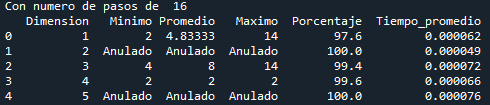
\includegraphics[width=80mm]{tiempo_pasos16.png}
\caption{\label{fig1}Caminata 16 pasos.}
\end{figure}
\begin{figure}[H]
\centering
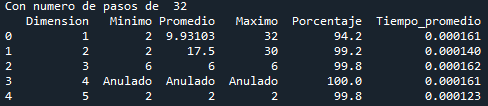
\includegraphics[width=80mm]{tiempo_pasos32.png}
\caption{\label{fig1}Caminata 32 pasos.}
\end{figure}
\begin{figure}[H]
\centering
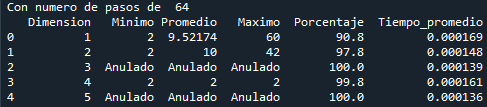
\includegraphics[width=80mm]{tiempo_pasos64.png}
\caption{\label{fig1}Caminata 64 pasos.}
\end{figure}
\begin{figure}[H]
\centering
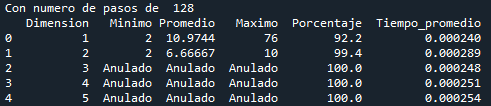
\includegraphics[width=80mm]{tiempo_pasos128.png}
\caption{\label{fig1}Caminata 128 pasos.}
\end{figure}
\begin{figure}[H]
\centering
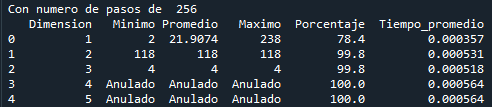
\includegraphics[width=80mm]{tiempo_pasos256.png}
\caption{\label{fig1}Caminata 256 pasos.}
\end{figure}
\begin{figure}[H]
\centering
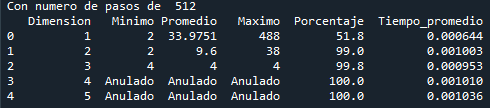
\includegraphics[width=80mm]{tiempo_pasos512.png}
\caption{\label{fig1}Caminata 512 pasos.}
\end{figure}


\section{Reto 2}
El segundo reto es realizar una comparación entre una implementación paralela y otra versión que no aproveche paralelismo en términos del tiempo de ejecución, aplicando alguna prueba estadística adecuada para determinar si la diferencia es significativa. [1]

Para este reto decidí convertir mi código original en una función para poder llamarlo con un def, dejando como varibale la dimensión para utilizar el multiprocessing.

\begin{verbatim}

from random import random,randint
import matplotlib.pyplot as plt
import multiprocessing

def practica1(dimension):

    for e in range (6):
        exponencial = e + 4
        exp= 2**exponencial
        print ('con numero de paso de', exp)
     
        
        pinicial = [0] * dimension
        res = []
        rep = 30
        
        
        for nr in range (rep) :
            nunca = True 
            
            
            for paso in range (exp):
                dim = randint(0,dimension-1)
                pinicial[dim]=pinicial[dim]+ 1 if random() < 0.5 else pinicial[dim] - 1
                
                if all ([p==0 for p in pinicial]):
                    res.append(paso)
                    nunca = False
                    
                    break
            if nunca:
                res.append(None)
        cuantos = sum([r is None for r in res])
        print ( cuantos/rep,'no regresaron nunca en la dimension', dimension)
        
        if cuantos < rep:
            regresaron = sum([r if r is not None else 0 for r in res])
            print (regresaron/(rep- cuantos), 'fue la tardanza en promedio en la dimensión', dimension)
            
if __name__ == "__main__":
     # practica1(2)
    # dimension = [d for d in range(1, 2)]
    # p = [(d) for d in dimension]
    # print(p, dimension)
    job=[]
    for i in range(1,6):
        p1 = multiprocessing.Process(target=practica1, args=(i,))
        job.append(p1)
        p1.start()
    # with multiprocessing.Pool() as pool:
    #     inicio = pool.map(practica1, p)
    # print(inicio)
   
\end{verbatim}

\begin{thebibliography}{99} %% use BibTeX or add references manually

\bibitem{ESchaeffer} Elisa Schaeffer. Práctica 1 Febrero 2021
\url{https://elisa.dyndns-web.com/teaching/comp/par/p1.html}.

\bibitem{ESchaeffer} Elisa Schaeffer. ejemplo caminata.py Febrero 2021
\url{https://github.com/satuelisa/Simulation/blob/master/BrownianMotion/caminata.R}.

\bibitem{Pandas} Ejemplo libreria Pandas
\url{https://www.geeksforgeeks.org/dealing-with-rows-and-columns-in-pandas-dataframe/}.

\end{thebibliography}

\end{document}
